\chapter{4. Métodos y herramientas}

En esta sección se describe los métodos, técnicas y herramientas tecnológicas empleados para el desarrollo del trabajo, así como los factores fundamentales que determinaron su elección y la incorporación dentro del proyecto. Se presentan además los entornos de desarrollo, los sistemas de control de versiones y las herramientas de documentación usadas para poner en marcha el sistema~\cite{pressman2005}.

\section{Métodos de desarrollo}

Durante la ejecución del proyecto se aplicó una perspectiva iterativa e incremental con influencias de metodologías ágiles. Esto permitió agrupar el trabajo en múltiples etapas y establecer un marco firme para la organización de la planificación, evaluación y mejora de las características adicionales añadidas~\cite{pressman2005}.

\subsection{Scrum}

Scrum es una metodología ágil orientada a administrar y elaborar proyectos de software. Su efectividad depende del uso de iteraciones llamadas \textit{sprints}, las cuales permiten la implementación de funciones del sistema.

En este proyecto se aplicó una variante modificada de la Scrum, subdividiendo el ciclo de desarrollo en segmentos cortos, con el fin de revisar el avance en cada momento. El enfoque adoptado facilitó la gestión estructurada de la incorporación de las nuevas funcionalidades y el corrección de los errores encontrados al desenvolver el sistema.

\subsection{Kanban}

Kanban es una metodología visual de gestión del trabajo diseñada para mejorar la fluidez de tareas y facilitar el control sobre el estado del proyecto. Utiliza tableros con columnas que corresponden a las distintas fases del proceso de desarrollo.

Durante el proyecto se ha empleado un sistema de organización basado en tableros Kanban mediante GitHub Projects, permitiendo gestionar tareas pendientes, funcionalidades en desarrollo y elementos completados de manera visual y estructurada~\cite{github}.

La Figura~\ref{fig:kanban_board} muestra el tablero Kanban utilizado durante el desarrollo del proyecto. Esta organización permitió visualizar el estado de las tareas, diferenciar el trabajo pendiente del trabajo en curso y mantener un seguimiento progresivo de las funcionalidades implementadas.

\begin{figure}[H]
    \centering
    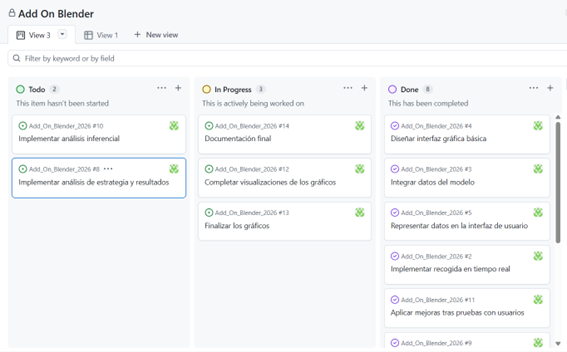
\includegraphics[width=0.9\textwidth]{diagramas/kanban.png}
    \caption{Tablero Kanban utilizado para la organización del desarrollo del proyecto.}
    \label{fig:kanban_board}
\end{figure}

\section{Tecnologías principales}

\subsection{Blender}

Blender se eligió porque cuenta con una arquitectura extendible y permite desarrollar funciones personalizadas con \textit{add-ons}. También ofrece acceso al código fuente de la escena tridimensional, lo que le permite supervisar eventos e informar datos relacionados con el proceso de modelado~\cite{blenderapi}.

\subsection{Python}

El lenguaje Python~\cite{pythonlang} ha sido usado en este trabajo debido a su integración nativa con Blender y a su amplio ecosistema de bibliotecas de datos y procesamiento automático. Con Python es posible implementar un sistema de captura de eventos, procesamiento de datos y generación de visualizaciones analíticas dentro del espacio tridimensional. A nivel de abstracción, Python posee flexibilidad que nos ayuda a construir entornos portables mediante directorios internos de paquetes (\textit{site-packages}). Esos directorios de paquetes pueden distribuirse sin interferir con la distribución global del software anfitrión y sus dependencias.

\subsection{Blender Python API (\texttt{bpy})}

Con el Blender Python API (\texttt{bpy})~\cite{blenderapi}, La API de Blender permite controlar la escena tridimensional, los objetos y las operaciones ejecutadas por el usuario.

A través de esta interfaz se accede a información relacionada con:
\begin{itemize}
\item Objetos y jerarquías de la escena activa.
\item Matrices de transformación espacial de coordenadas mundiales y locales.
\item Topología estructural de mallas mediante punteros nativos y submodelos \textit{BMesh}.
\item Modos de trabajo y conmutación de la interfaz gráfica.
\item Eventos y operadores ejecutados en el flujo de ejecución del usuario.
\end{itemize}

Asimismo, la API permite implementar sistemas de monitorización mediante la suscripción de funciones a los \textit{handlers} de la aplicación, utilizados para detectar automáticamente modificaciones analíticas durante las sesiones de modelado.

La Figura~\ref{fig:api_blender} representa de forma esquemática la interacción entre Blender, la API \texttt{bpy} y los módulos desarrollados. Esta relación es fundamental para comprender cómo el sistema accede a la escena, detecta operaciones del usuario y conecta la captura de datos con el posterior análisis.

\begin{figure}[H]
    \centering
    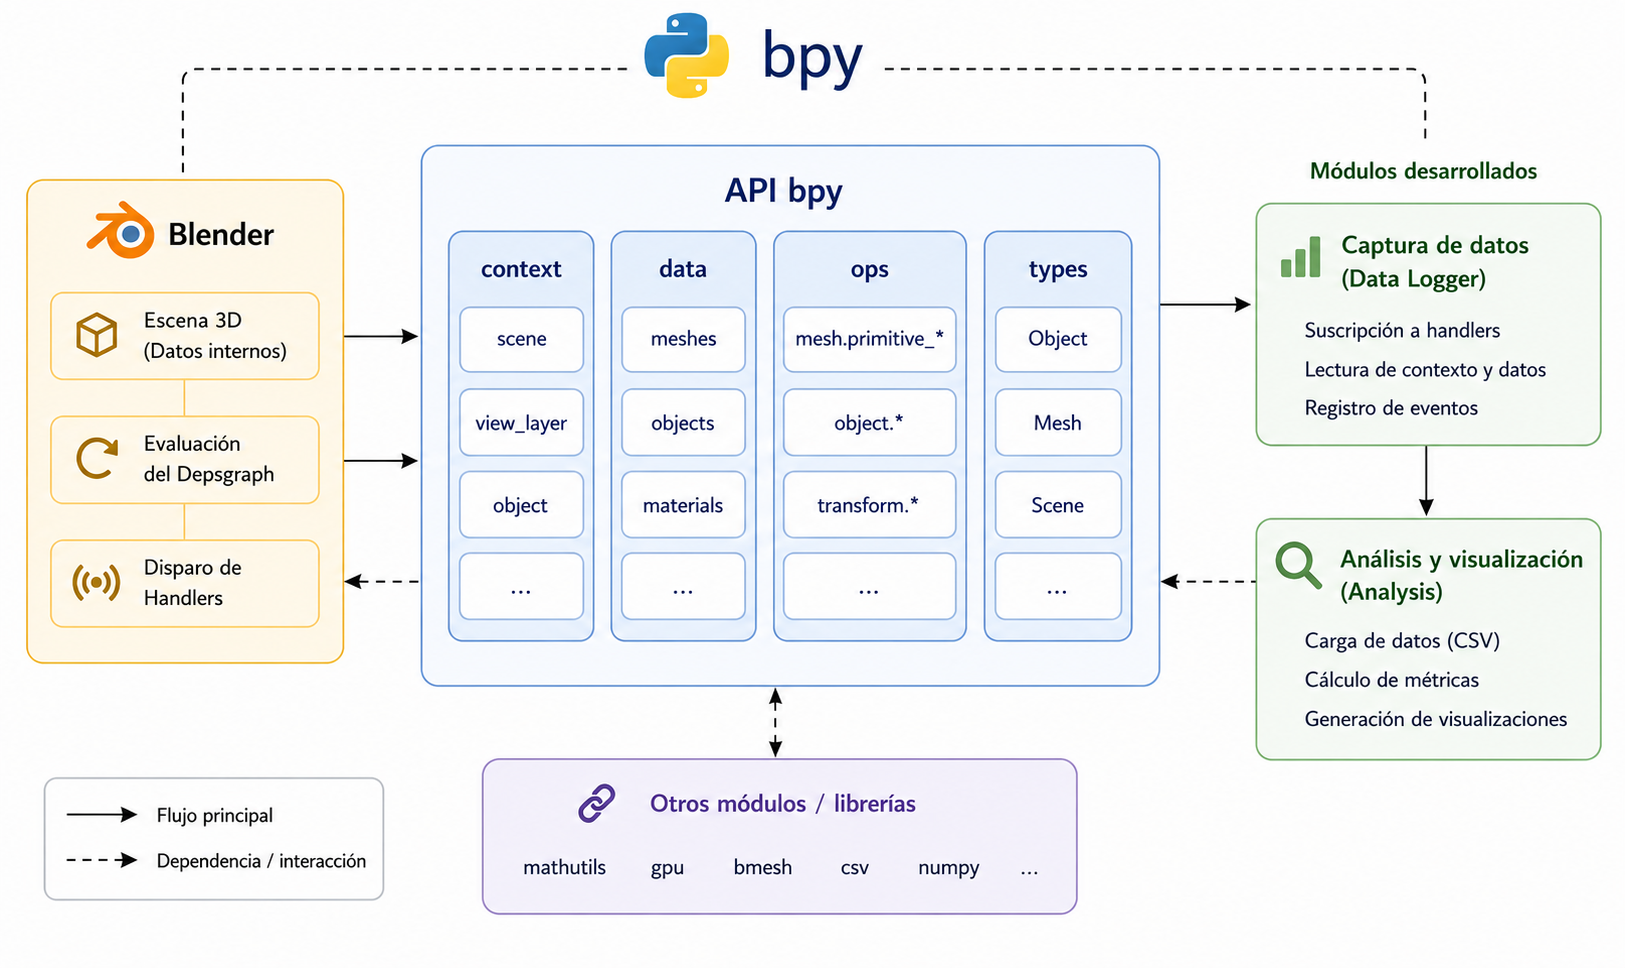
\includegraphics[width=0.9\textwidth]{diagramas/interaccion_api.png}
    \caption{Esquema conceptual de interacción entre Blender, la API bpy y los módulos desarrollados}
    \label{fig:api_blender}
    {\footnotesize \textit{Nota. Figura elaborada por la autora con asistencia de ChatGPT.}}
\end{figure}

\subsection{Persistencia de datos en formato CSV}

El formato CSV (\textit{Commas-Separated Values}) ha servido como la base para registrar el registro secuencial de las interacciones~\cite{mckinney2022python}.

Este método de uso es razonable ya que es simple, técnicomente compatible, minimalista en el manejo de la memoria volátil y fácil de integrar con herramientas externas de análisis. Para mejorar la velocidad de acceso y la persistencia, mientras no afecta al rendimiento del visor 3D en tiempo real, el procesamiento de dichos archivos tabulados se realiza mediante flujos lineales con diccionario orientados, utilizando el módulo \texttt{csv.DictReader} nativo para evitar la sobreexplotación de la memoria con bibliotecas masivas de análisis de datos.

La Figura~\ref{fig:csv} muestra de forma resumida un archivo csv generado por el \textit{add-on} de detección de datos.

\begin{figure}[H]
    \centering
    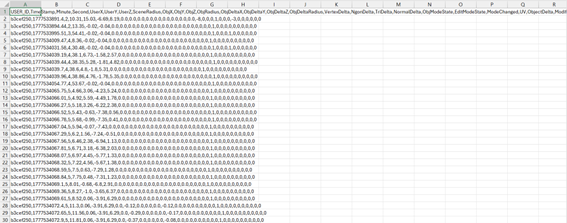
\includegraphics[width=0.9\textwidth]{diagramas/csv_example.png}
    \caption{Ejemplo de estructura de datos en formato CSV generada de forma automatizada por el sistema.}
    \label{fig:csv}
\end{figure}

\subsection{NumPy}

NumPy constituye una biblioteca especializada en computación numérica y procesamiento eficiente de estructuras matriciales en Python. Su utilización es crítica en este sistema para realizar operaciones vectoriales de alto rendimiento, el cálculo de las posiciones espaciales de los vértices evaluados y las transformaciones numéricas necesarias para proyectar los datos estadísticos sobre el espacio geométrico bidimensional y tridimensional~\cite{mckinney2022python}.

\subsection{BMesh y mathutils}

La biblioteca \texttt{bmesh} se ha utilizado para acceder a la representación editable de las mallas de Blender. Su uso resulta especialmente relevante en operaciones de análisis topológico, recuento de caras, cálculo de islas UV y consulta de aristas compartidas entre caras. Esta capa proporciona un control más preciso que la estructura \texttt{Mesh} evaluada cuando el usuario trabaja en modo edición~\cite{botsch2010polygon,blenderapi}.

El módulo \texttt{mathutils} se ha empleado para operar con vectores, matrices y transformaciones espaciales. Gracias a estas estructuras se calculan centros de objetos, radios de escena, coordenadas globales, desplazamientos y comparaciones geométricas entre modelos.

\subsection{Matplotlib y Renderizado en Memoria por Canales}

Matplotlib~\cite{matplotlib} se ha empleado para la generación de las representaciones gráficas y visualizaciones de carácter inferencial y descriptivo.

A diferencia de los entornos de ejecución tradicionales de análisis científico, donde los gráficos se despliegan en ventanas independientes del sistema operativo a través de interfaces de usuario bloqueantes, en esta solución se implementa una técnica de desacoplamiento basada en el motor de renderizado abstracto de la biblioteca (\texttt{FigureCanvasAgg}). Esto permite generar los diagramas estadísticos y las matrices de correlación directamente en un espacio de memoria volátil como matrices de píxeles (\textit{raw buffers}), las cuales son inyectadas dinámicamente como texturas en tiempo de ejecución sobre mallas poligonales procedurales en el visor 3D de Blender~\cite{munzner2014visualization}.

\section{Herramientas de desarrollo}

\subsection{Visual Studio Code}

Visual Studio Code ha sido utilizado como entorno de desarrollo principal durante la implementación del proyecto. Este editor proporciona herramientas avanzadas de depuración de hilos, autocompletado sintáctico y gestión de extensiones, facilitando el desarrollo de código en Python y la integración con sistemas de control de versiones~\cite{pep8,vscode}.

\subsection{Git y GitHub}

Git ha sido empleado como sistema de control de versiones para gestionar el historial de cambios al desarrollarse el proyecto~\cite{git}. Además, GitHub se ha utilizado como plataforma de alojamiento remoto del repositorio, lo que permite almacenar versiones del código, gestionar ramas de desarrollo y mantener un seguimiento bien ordenado del progreso del sistema~\cite{github}.

\subsection{GitHub Projects}

GitHub Projects se ha empleado como herramienta de organización y planificación de tareas mediante tableros Kanban. Su utilización ha permitido estructurar el flujo de trabajo y mantener un seguimiento visual del estado de desarrollo de cada funcionalidad implementada.

\subsection{Overleaf y entornos locales de LaTeX}

La memoria del proyecto ha sido desarrollada usando \LaTeX{} —un sistema de composición tipográfica muy popular en documentos científicos y técnicos—~\cite{wiki:latex}. Inicialmente, se utilizaron las plataformas web Overleaf para la edición y la comprensión colaborativa del documento~\cite{overleaf}. Tras la creciente demanda de imágenes y la subida de la complejidad técnica, el proceso principal se transferió a un entorno local de composición tipográfica para asegurar que el tiempo de elaboración del documento final fuera óptimo.

\begin{table}[H]
\centering
\small
\setlength{\tabcolsep}{4pt}
\renewcommand{\arraystretch}{1.15}
\begin{tabularx}{\textwidth}{Xcccc}
\toprule
\textbf{Herramientas} & 
\textbf{Desarrollo} & 
\textbf{Procesamiento} & 
\textbf{Visualización 3D} & 
\textbf{Memoria} \\
\midrule
Python                      & X & X & X &   \\
Blender API (\texttt{bpy})  & X &   & X &   \\
BMesh                       & X & X &   &   \\
\texttt{mathutils}          & X & X & X &   \\
Formatos CSV                & X & X &   &   \\
NumPy                       &   & X & X &   \\
Matplotlib                  &   & X & X &   \\
Visual Studio Code          & X &   &   &   \\
Git                         & X & X & X & X \\
GitHub                      & X & X & X & X \\
Blender                     & X &   & X &   \\
Overleaf                    &   &   &   & X \\
LaTeX                       &   &   &   & X \\
\bottomrule
\end{tabularx}
\caption{Herramientas y tecnologías utilizadas en el desarrollo del proyecto.}
\label{tab:herramientas}
\end{table}
